\chapter{A Brief Guide}
\label{chap:guide}

\section{What is \LaTeX{}} % (fold)

\LaTeX{} (pronounced "Lah-tech" or "Lay-tech") is a macro package created by Leslie Lamport based on \TeX{}. As a document preparation system for high-quality typesetting in almost any forms of publishing, \LaTeX{} is not the name of a particular editing program, but refers to the encoding or tagging conventions that are used in \LaTeX{} documents \citep{website:wikipedia,website:latex}.

% section What is \LaTeX{} (end)

\section{Why use \LaTeX?}

There are a lot of good reasons why you need to use \LaTeX{}, the most significant one is the following:
\begin{itemize}
    \item Allows you to clearly separate the content from the format of your document.
    \item Let you concentrate on your ideas, not visual appearance!
\end{itemize}

You can concentrate purely on the structure and contents of your document, not superficial layout issues. You don't need to manually adjust fonts, text sizes, line heights, or text flow for readability, as \LaTeX{} takes care of them automatically. \citep{website:wikibook}
\begin{figure}[!htbp]
    \centering
    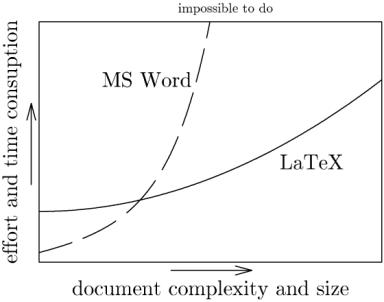
\includegraphics[width=0.6\textwidth]{compare}
    \caption{Comparison between Microsoft Word and \LaTeX{} [From Google Images]}
    \label{fig:compare}
\end{figure}

\section{How to use?} % (fold)

\subsection{Installation} % (fold)
LaTeX is based on open-source code, so it is available on most computing platforms as free software.
\begin{itemize}
    \item Linux: TeXLive distribution. 
    \item MacOS: Mactex or TeXLive.
    \item Windows: MikTeX or TeXLive. 
\end{itemize}

Note: the best resource that can be used to learn \LaTeX{} is "\LaTeX{} Wikibook", which is available online.

Note: to use \LaTeX{}, you need a text editor for writing and editing ".tex" files. To open the ".tex" files in this template, you need a text editor which supports "UTF-8" encoding. Free options for different platforms are following:
\begin{itemize}
    \item Linux: vim. 
    \item MacOS: TeXShop, Macvim.
    \item Windows: Texmaker, Gvim, Notepad++. 
\end{itemize}
% subsection Installation (end)

\subsection{Give a try} % (fold)
After downloading this template and installing a \LaTeX{} distribution. It's time to have a try:
\begin{itemize}
    \item Linux: run Compile.sh
    \item MacOS: run Compile.sh
    \item Windows: run Compile.bat
\end{itemize}

Note: It's recommended to use the provided scripts to compile your \LaTeX{} files. It will automatically search and include files without explicitly specifying relative paths. If you do not use them for compilation, you need to specify the relative path in each "\verb+\input{ }+" command, or the \LaTeX{} will complain that it can not find some files.

Note: the bash script "Compile.sh" hasn't been tested on MacOS. If there are some errors, please give me your feedback, thank you so much.

% subsection Give a try (end)

\subsection{Include math} % (fold)
\LaTeX{} realization of Equation~\ref{eq:N-S_equation} is something like this:
\begin{center}
    \small
    \begin{verbatim}
    \begin{equationa}\label{eq:N-S_equation}
        \frac{\partial (\rho\mathbf{v})}{\partial t} +
        \nabla \cdot (\rho \mathbf{v} \mathbf{v}) =
        -\nabla p + \nabla \cdot\mathbf{T} + \mathbf{f}. 
    \end{equation}    
\end{verbatim}
\end{center}

\begin{equation}\label{eq:N-S_equation}
    \frac{\partial (\rho\mathbf{v})}{\partial t} + \nabla \cdot (\rho \mathbf{v} \mathbf{v}) = -\nabla p + \nabla \cdot\mathbf{T} + \mathbf{f}. 
\end{equation}    
% subsection Include math (end)

\subsection{Include Graphics} % (fold)
Note: inluding figures may seem to be scary by looking at the codes. However, the fact is that you only need to modify the names in each part, the rest are simply copy and paste! These codes are all available in the file "Useful Commands.txt".

Figure~\ref{fig:ITC_Q_Criteria} is an example for including a single figure.
\begin{center}
    \small
    \begin{verbatim}
        \begin{figure}[!htbp]
            \centering
            \includegraphics[width=\MyFactor\textwidth]{ITC_Q_Criteria}
            \caption{An Example for including a single figure}
            \label{fig:ITC_Q_Criteria}
        \end{figure}
    \end{verbatim}
\end{center}

Figure~\ref{fig:HC_OASPL} is an example for including multiple figuress. 
\begin{figure}[!htbp]
    \centering
    \includegraphics[width=\MyFactor\textwidth]{ITC_Q_Criteria}
    \caption{An Example for including a single graph}
    \label{fig:ITC_Q_Criteria}
\end{figure}
\begin{center}
    \small
    \begin{verbatim}
        \begin{figure}[!htbp]
            \centering
            \begin{subfigure}[b]{\MySubFactor\textwidth}
                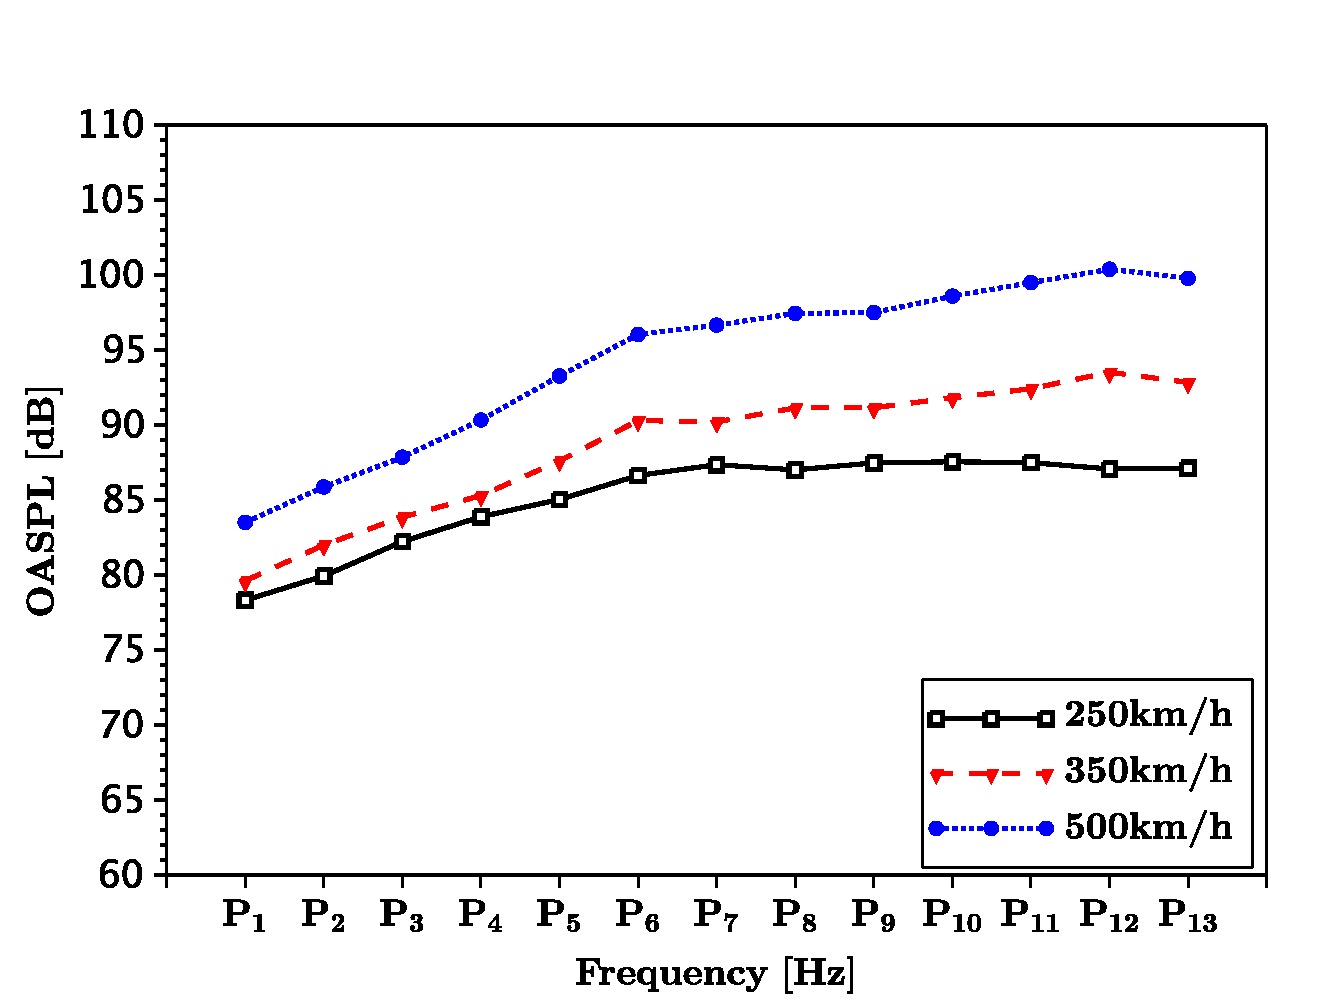
\includegraphics[width=\textwidth]{HC_OASPL_A}
                \caption{}
                \label{fig:HC_OASPL_A}
            \end{subfigure}%
            ~% add a small space
            \begin{subfigure}[b]{\MySubFactor\textwidth}
                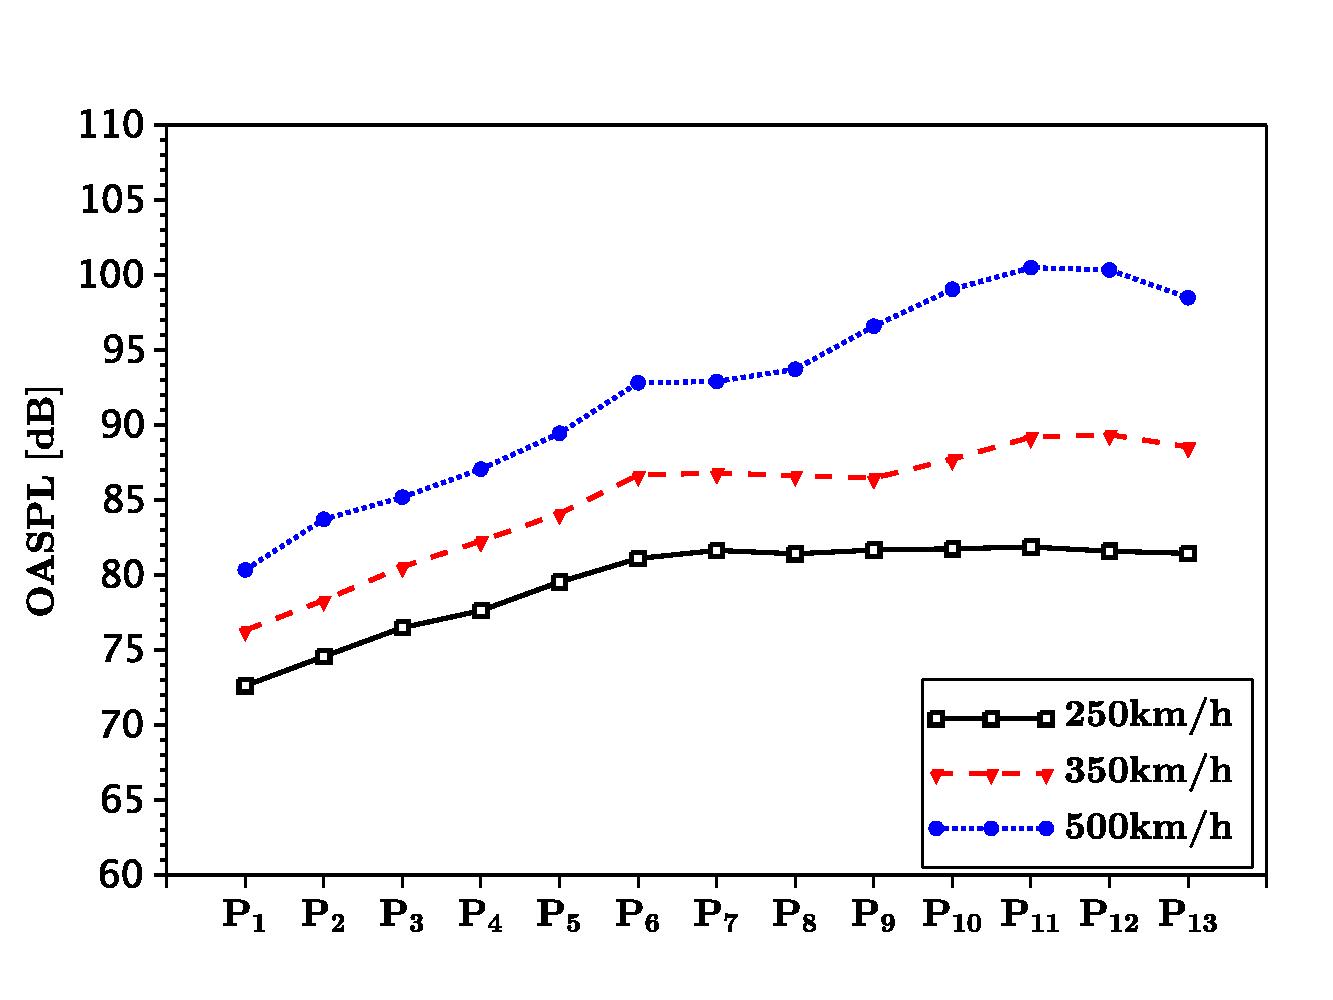
\includegraphics[width=\textwidth]{HC_OASPL_B}
                \caption{}
                \label{fig:HC_OASPL_B}
            \end{subfigure}%
            \\% change line
            \begin{subfigure}[b]{\MySubFactor\textwidth}
                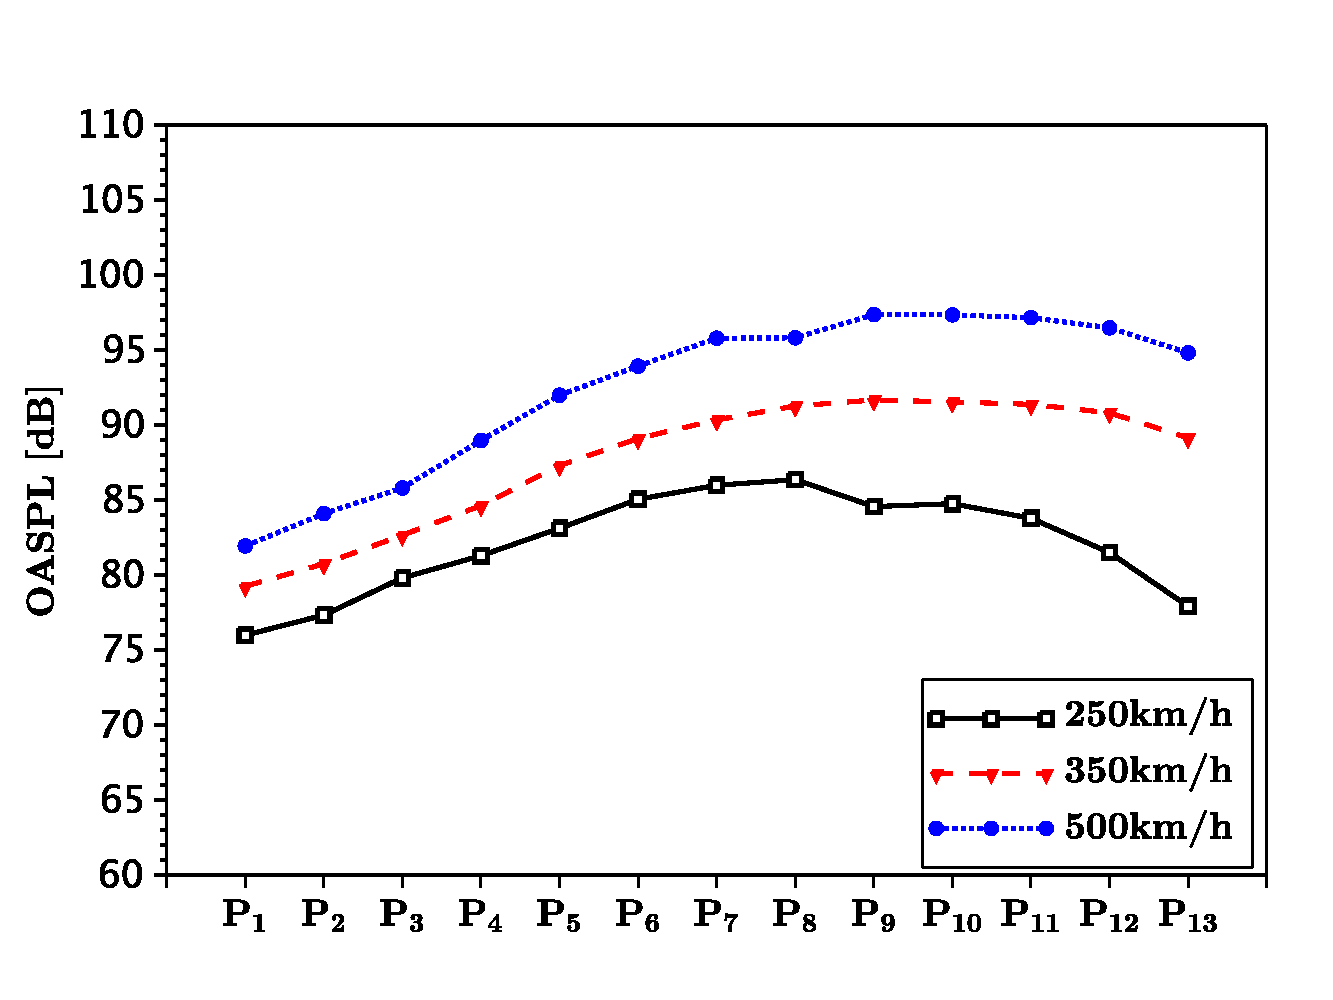
\includegraphics[width=\textwidth]{HC_OASPL_C}
                \caption{}
                \label{fig:HC_OASPL_C}
            \end{subfigure}%
            ~% add a small space
            \begin{subfigure}[b]{\MySubFactor\textwidth}
                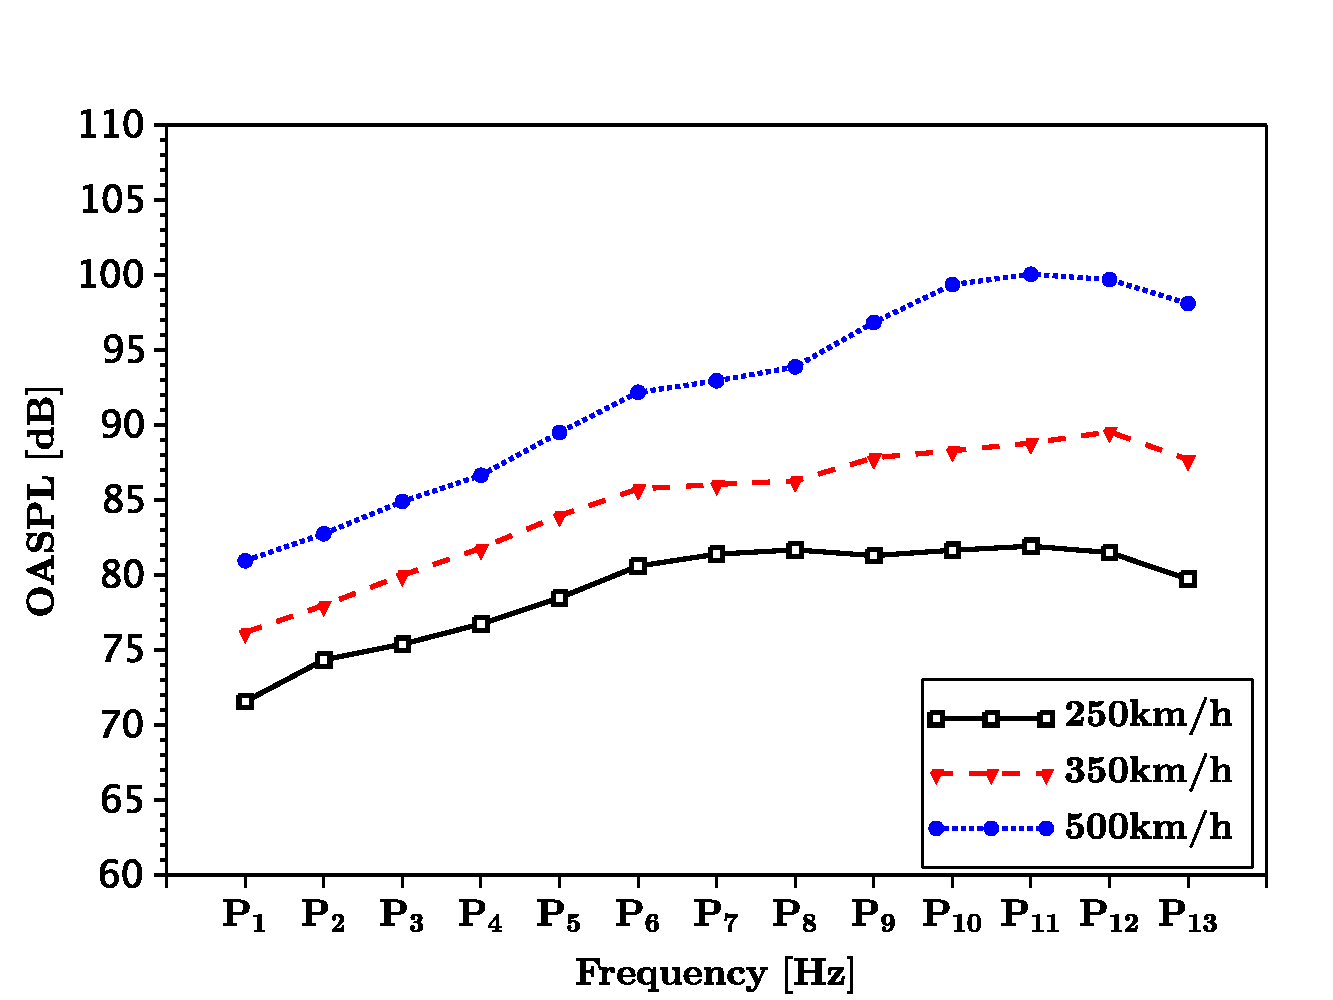
\includegraphics[width=\textwidth]{HC_OASPL_D}
                \caption{}
                \label{fig:HC_OASPL_D}
            \end{subfigure}%
            \caption{An Example for including multiple figures}
            \label{fig:HC_OASPL}
        \end{figure}
    \end{verbatim}
\end{center}
\begin{figure}[!htbp]
    \centering
    \begin{subfigure}[b]{\MySubFactor\textwidth}
        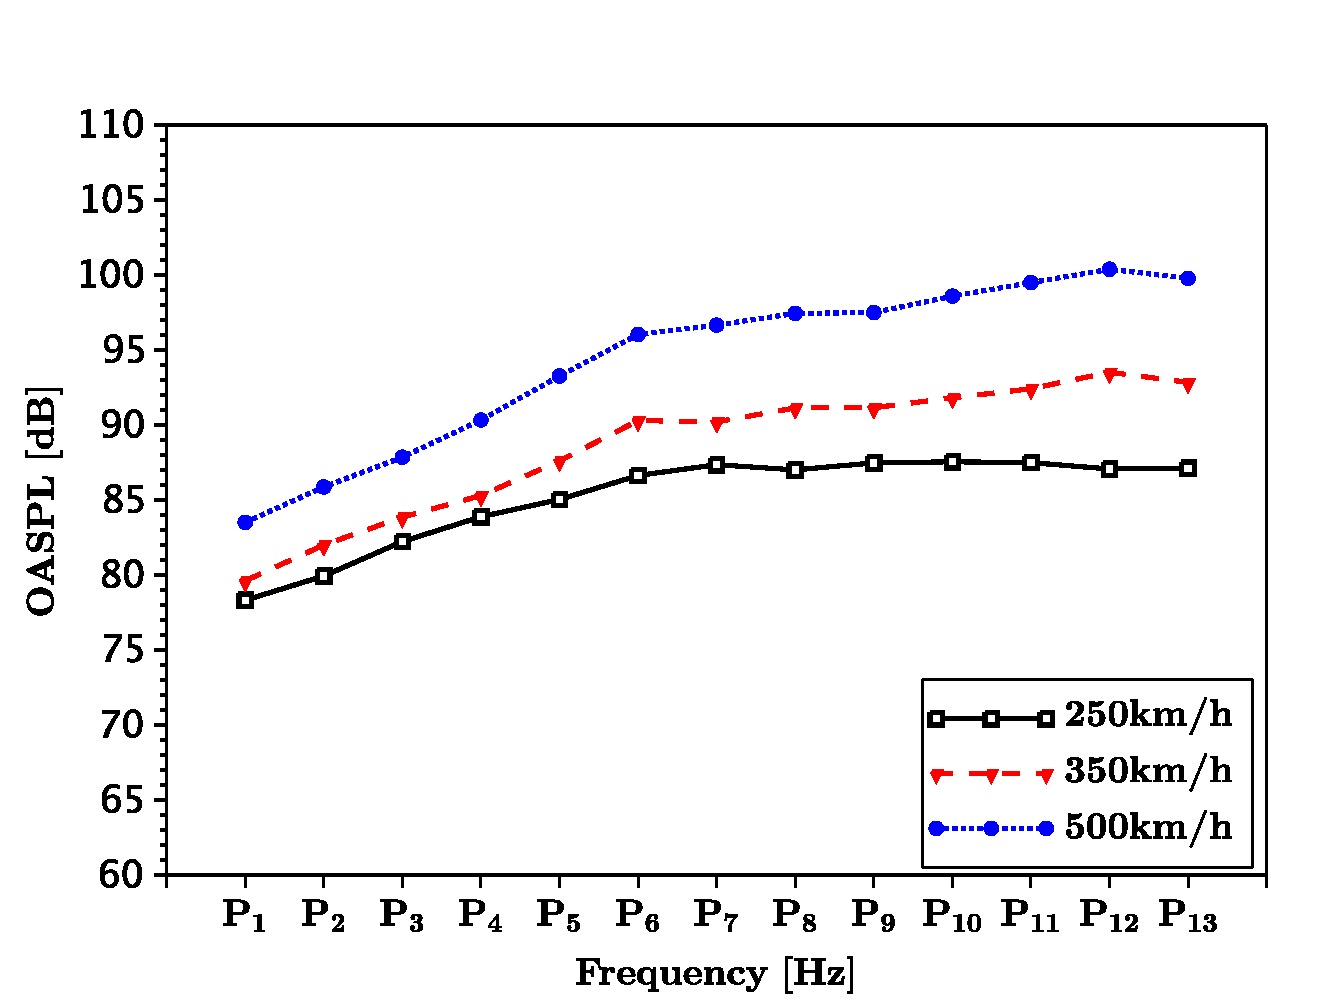
\includegraphics[width=\textwidth]{HC_OASPL_A}
        \caption{}
        \label{fig:HC_OASPL_A}
    \end{subfigure}%
    ~% add a small space
    \begin{subfigure}[b]{\MySubFactor\textwidth}
        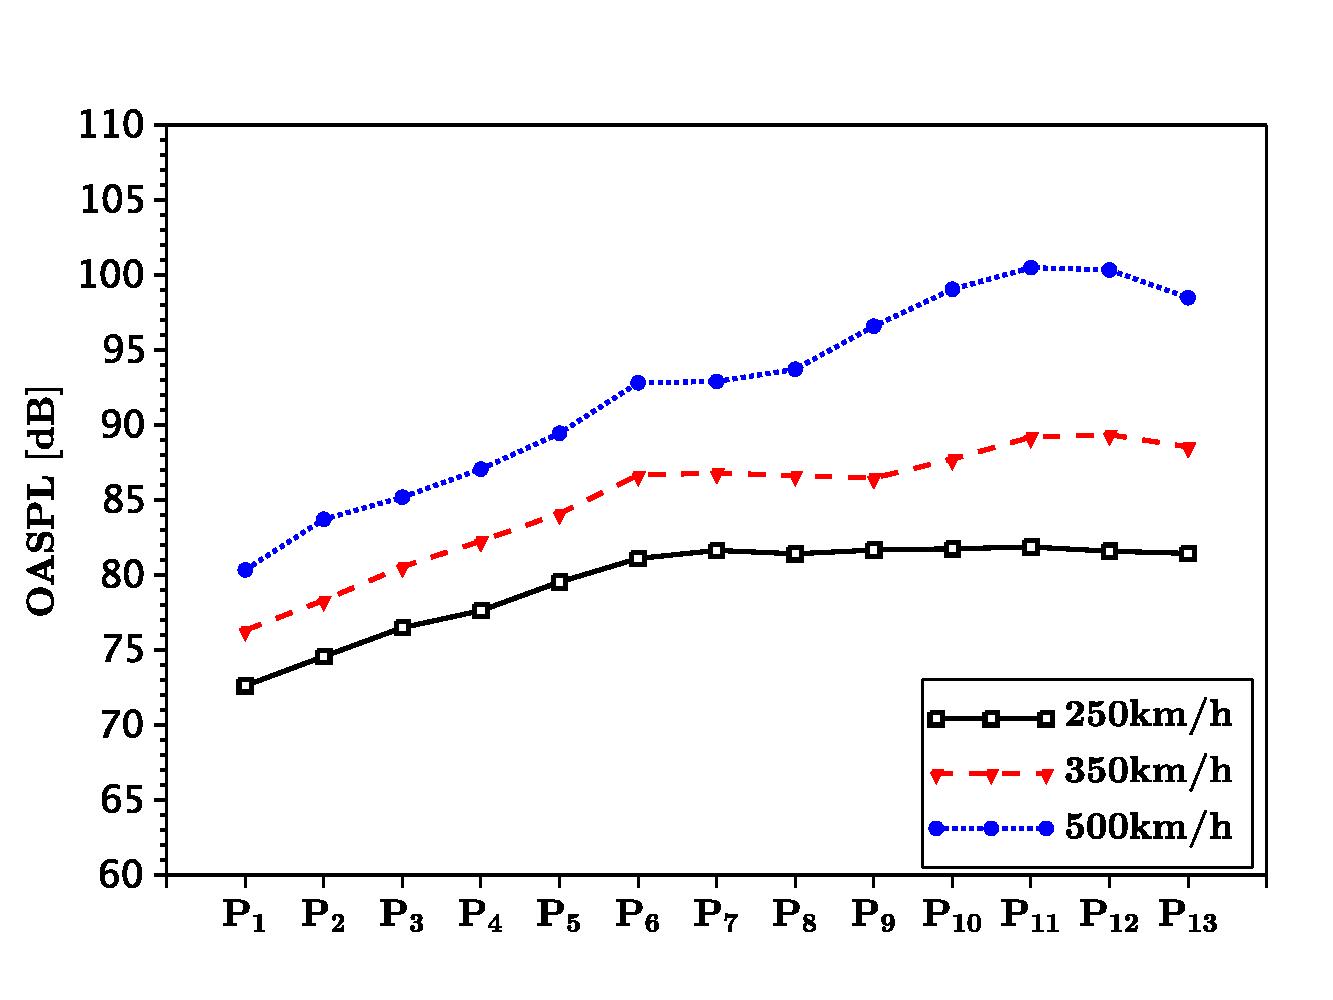
\includegraphics[width=\textwidth]{HC_OASPL_B}
        \caption{}
        \label{fig:HC_OASPL_B}
    \end{subfigure}%
    \\% change line
    \begin{subfigure}[b]{\MySubFactor\textwidth}
        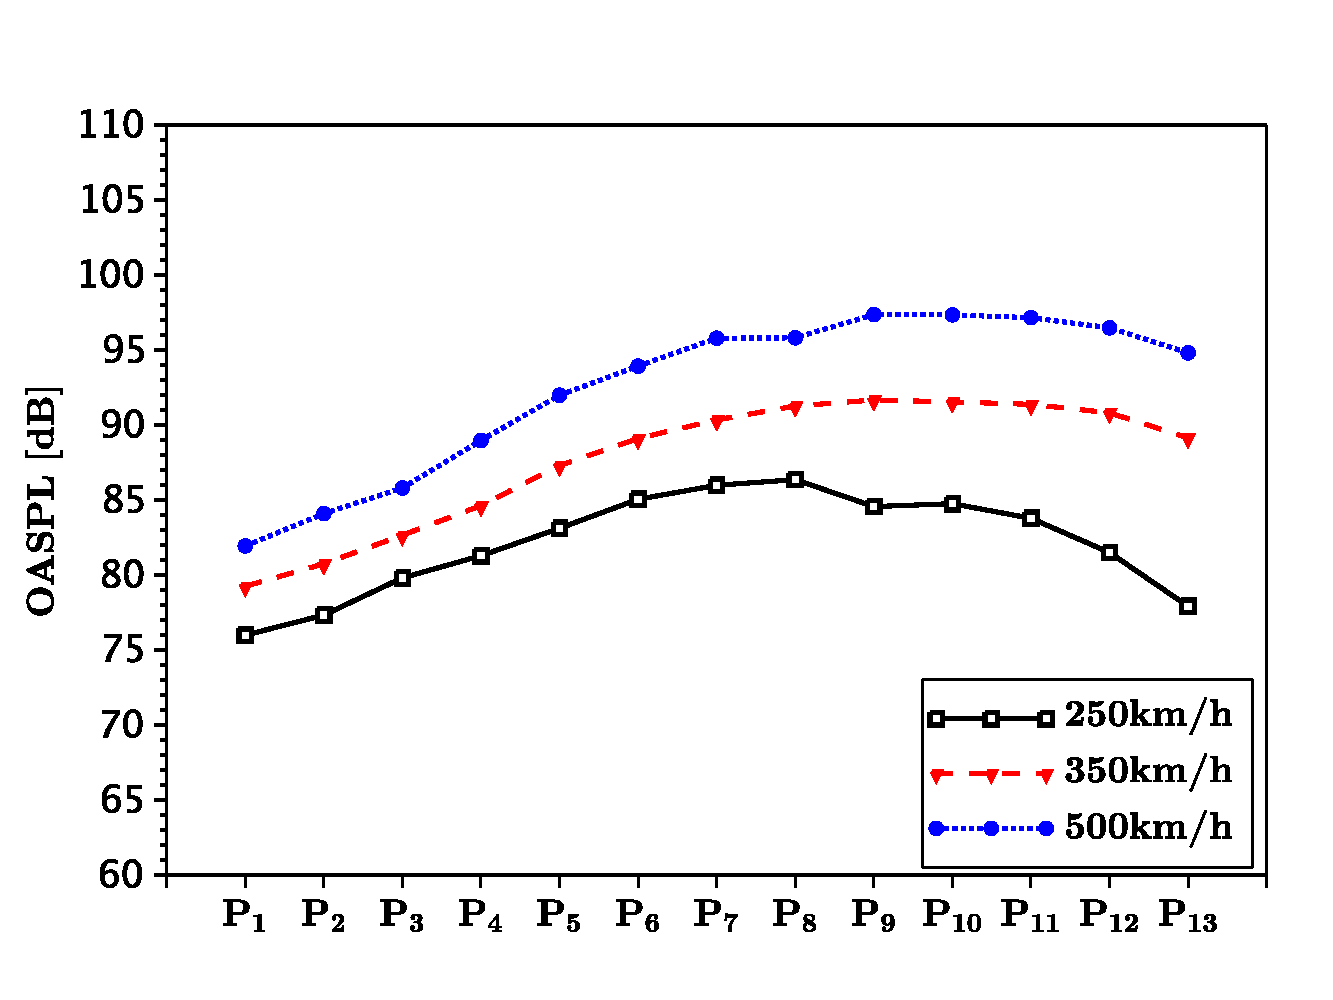
\includegraphics[width=\textwidth]{HC_OASPL_C}
        \caption{}
        \label{fig:HC_OASPL_C}
    \end{subfigure}%
    ~% add a small space
    \begin{subfigure}[b]{\MySubFactor\textwidth}
        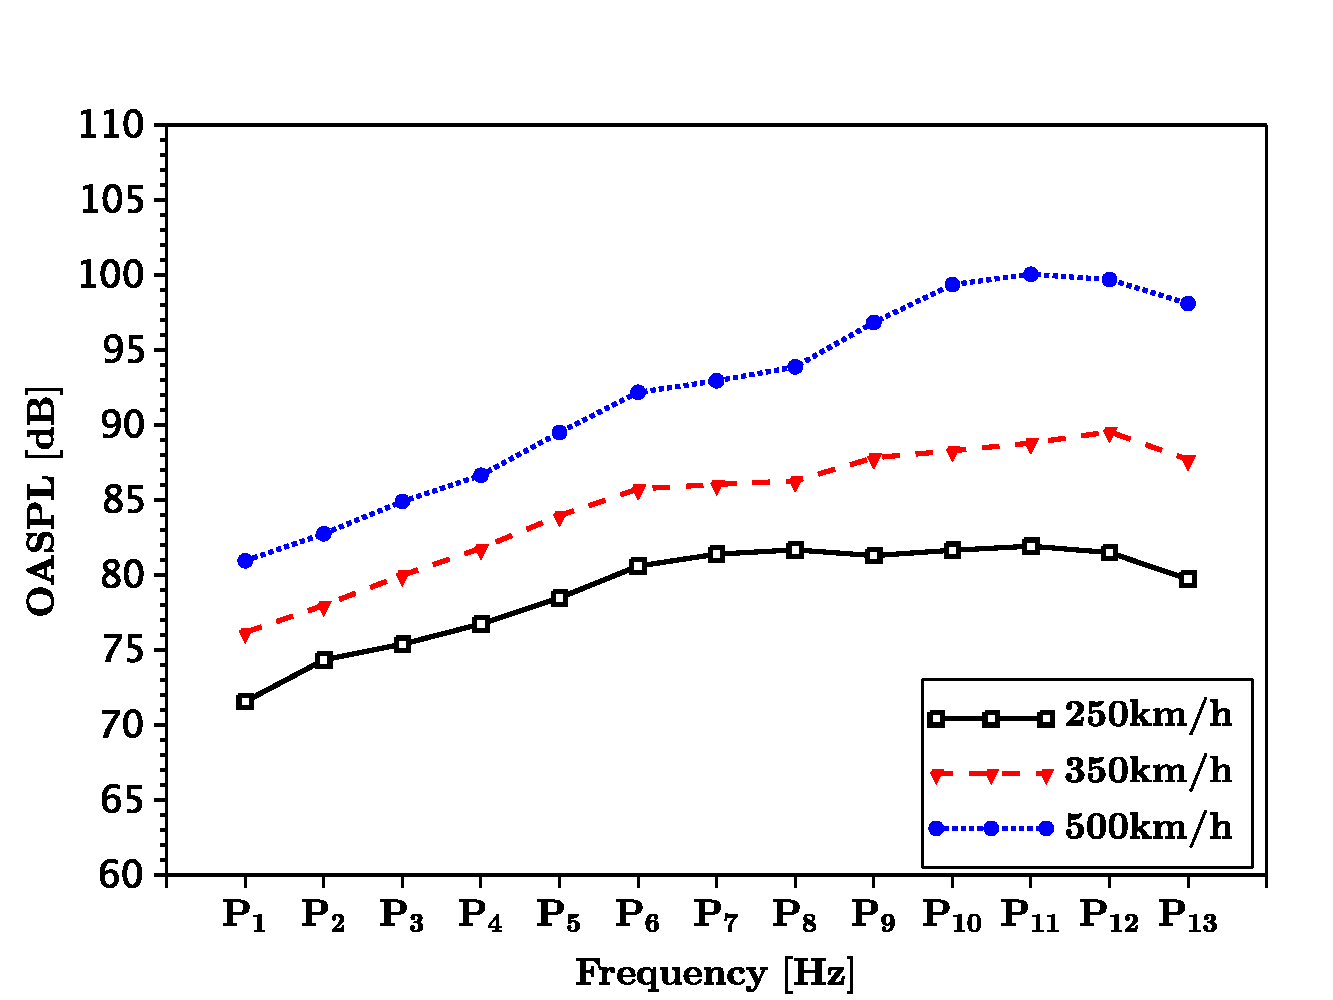
\includegraphics[width=\textwidth]{HC_OASPL_D}
        \caption{}
        \label{fig:HC_OASPL_D}
    \end{subfigure}%
    \caption{An Example for including multiple figures}
    \label{fig:HC_OASPL}
\end{figure}
% subsection Include Graphics (end)

\subsection{Include a citation} % (fold)
Suppose you are going to cite an article named "Document Preparation System", the procedures are:
\begin{itemize}
    \item Use Google Scholar search "Document Preparation System".
    \item Open "Cite" and choose "Import to Bibtex" under the target item.
    \item Copy the citation information of this article into the file "Myrefs.bib"
    \item Research dominant: cite this article by \verb+\citep{lamport1986document}+ like here \citep{lamport1986document}
    \item Citation dominant: cite this article by \verb+\citet{lamport1986document}+ like here \citet{lamport1986document}
    \item References list is generated automatically.
\end{itemize}
% subsection Include a citation (end)
\subsection{Generate nomenclature} % (fold)
In this template, a simple command for add nomenclatures is provided. Therefore, packages for automatical nomenclature generation are not included. From my point of view, there is no need to use those packages and make things complicated. However, if you insist, there are a lot of available packages for creating nomenclatures. Recommended options are (Please Google the one you want to know):
\begin{itemize}
    \item listofsymbols
    \item nomencl
\end{itemize}
% subsection Generate nomenclature automatically (end)
% section How to use? (end)

\section{File Tree of Current Template} % (fold)
\begin{itemize}
    \item Thesis.tex: main tex file, which acts like the main function in C++. No need to modify.
    \item Style: Store template configuration files, which act like subfunctions, No need to modify.
    \item Tmp: Store files generated by compilation.
    \item Biblio: Store information of references.
    \item Img: Store images.
    \item Tex: Store files for your content, this is the working directory.
        \begin{itemize}
            \item Frontpages: content of front pages, like authorship, abstract, etc.
            \item Prematter: content of nomenclature, etc.
            \item Main$\_$Content: index for chapters you want to include into your current content.
            \item Chap$\_$***: your content for each chapters.
            \item Appendix: appendix.
            \item Useful Commands: collection of useful commands.
        \end{itemize}
\end{itemize}

Note: this template can be easily adapted to other writing purposes such as articles. What you need to do is to change and adjust a few items in the "Thesis.tex" file, which would be very easy after you are a little familiar with using \LaTeX{}. Like :

Change \verb+\documentclass{uwaterloothesis}+ to \verb+\documentclass{article}+
% section File Tree of Current Template (end)

\section{Feedback and Problems} % (fold)
Please feel free to send me emails for any related problems:
\begin{center}
huangrui.mo@uwaterloo.ca
\end{center}
% section Feedback and Problems (end)
%%%%% ++++++++++++++++++++++++++++++++++++++++++++++++++++++++++++++++++++++++++++++
%%%%% ++++++++++++++++++++++++++++++++++++++++++++++++++++++++++++++++++++++++++++++
